\chapter{Аналитический раздел}
\label{cha:analysis}
%
% % В начале раздела  можно напомнить его цель
%
Алгоритмы, с которыми приходится иметь дело при параллельном программировании гораздо сложнее, чем аналогичные последовательные алгоритмы. Часть проблем касается распараллеливания самого алгоритма (например, как разбить процесс на задачи и как поставить им в соответствие физические процессоры), часть касается оптимального использования вычислительных ресурсов (баланс загрузки процессоров, межпроцессные взаимодействия, доступ к кэшу). Для разработки высокопроизводительных приложений программисту не только очень хорошо знать структуру самого приложения, но и структуру аппаратной платформы, а зачастую и программной (особенности операционной системы, компилятора и.т.д.).
Итак, уровень знаний, необходимый для разработки высокопроизводительных параллельных программ выше, чем для последовательных программ. Параллельное программирование может быть очень мучительным и запутанным. В добавок отладка параллельной программы и поиск критических мест также трудоёмкий и длительный процесс.
Из-за этих причин программирование для массивно параллельных машин считается непростым делом, и в значительной степени причиной этому служит недостаток инструментария по сравнению с последовательными машинами. Для того, чтобы понять поведение и внутреннюю логику параллельных программ и помочь программисту выявить потенциальные слабые места (например, ограничения по межпроцессным взаимодействиям) необходимы средства контроля хода выполнения параллельной программы. Они могут использоваться для сравнения производительности схожих программ или помогать при отладке.


% Обратите внимание, что включается не ../dia/..., а inc/dia/...
% В Makefile есть соответствующее правило для inc/dia/*.pdf, которое
% берет исходные файлы из ../dia в этом случае.



\section{Парадигмы параллельного программирования}
\subsection{Структура и характеристики параллельных алгоритмов}
Любой параллельный алгоритм (программа) состоит из блоков последовательных и параллельных вычислений. Последовательная часть программы (называется критическим сечением) – это последовательность операторов, которая должна выполняться только одним процессором. За критическим сечением обычно следует ветвление, инициирующее параллельно выполняемые участки программы (параллельные сегменты). В месте соединения параллельных сегментов выполняется синхронизация и параллельные сегменты возвращаются к критическому сечению. Синхронизация требуется для того, чтобы вычисления в параллельных сегментах закончились прежде, чем начнется выполнение последовательной части. 

\subsection{Программные парадигмы}

При параллельном программировании появляются дополнительные сложности (по сравнению с последовательным программированием): возникает необходимость управлять несколькими процессорами и координировать межпроцессорные вызовы. В общем случае параллельная программа представляет собой ряд заданий, работающих параллельно друг другу и взаимодействующих между собой. Существует несколько парадигм (моделей) программирования при создании параллельных алгоритмов. Наиболее распространенными парадигмами являются модель передачи сообщений и модель разделяемой памяти.


\subsection{Проектирование параллельных алгоритмов}
Несмотря на то, что проектирование параллельных алгоритмов есть процесс творческий и в общем случае достаточно сложно рекомендовать универсальный рецепт, следует все же привести общую методологию проектирования параллельных алгоритмов, которая в значительной степени оградит проектировщика от потенциальных ошибок.

\begin{figure}[h!]
	\centering
	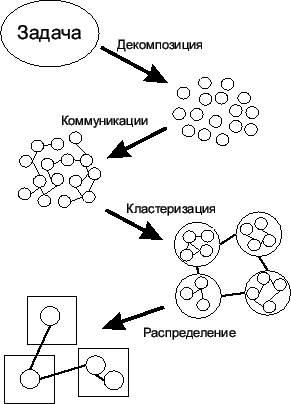
\includegraphics[width=0.4\textwidth]{img/img1.png}
	\caption{Методология проектирования параллельных алгоритмов}
	\label{fig:spire05}
\end{figure}

Описываемая методология проектирования предлагает подход к распараллеливанию, который рассматривает машинно-независимые аспекты реализации алгоритма, такие как параллелизм, на первой стадии, а особенности проектирования, связанные с конкретным параллельным компьютером, - на второй. Данный подход разделяет процесс проектирования на четыре отдельных этапа: декомпозиция (partitioning), коммуникации (communications), кластеризация (agglomeration) и распределение (mapping). Первые два этапа призваны выделить в исходной задаче параллелизм и масштабируемость, остальные этапы связаны с различными аспектами производительности алгоритма\cite{test1_B}. Рисунок 1.1 иллюстрирует процесс проектирования параллельного алгоритма.  
Сформулируем кратко содержание этих этапов. 
\subsubsection{Декомпозиция} 
Общая задача вычислений и обработки данных делится на меньшего размера подзадачи. При этом игнорируются проблемы практической реализации, например, число процессоров используемого в будущем компьютера. Напротив, все внимание сосредотачивается на возможном параллелизме исходной задачи. 
\subsubsection{Коммуникации}
Определяется требуемая связь между подзадачами, ее структура и конкретные алгоритмы коммуникаций. 
\subsubsection{Кластеризация} 
Структура подзадач и коммуникаций оценивается с учетом требований производительности алгоритма и затрат на реализацию. Если необходимо, отдельные подзадачи комбинируются в более крупные с целью улучшения производительности и снижения затрат на разработку. 
\subsubsection{Распределение} 
Каждая подзадача назначается определенному процессору, при этом стараются максимально равномерно загрузить процессоры и минимизировать коммуникации. Распределение может быть статическим или формироваться в процессе выполнения программы на основе алгоритмов балансировки загрузки (load balancing algorithms). 
Следует заметить, что при прохождении последних двух этапов необходимо учитывать архитектуру параллельного компьютера, имеющегося в распоряжении разработчика, другими словами параллельный алгоритм должен быть адекватен используемой параллельной системе. 

\subsection{Характеристики производительности параллельного алгоритма}
Задачей программиста является проектирование и реализация программ, которые удовлетворяют требованиям пользователя в смысле производительности и корректной работы. Производительность является достаточно сложным и многосторонним понятием. Кроме времени выполнения программы и масштабируемости следует также анализировать механизмы, отвечающие за генерацию, хранение и передачу данных по сети, оценивать затраты, связанные с проектированием, реализацией, эксплуатацией и сопровождением программного обеспечения. Существуют весьма разнообразные параметры, влияющие на производительность вычислительной системы. Среди них наиболее значимыми являются: требования по памяти, производительность сети, время задержки при передаче данных (latency time), переносимость, масштабируемость, затраты на проектирование, реализацию, отладку, требование к аппаратному обеспечению и т.д. Критериями, по которым оценивается производительность, являются время выполнения программы, ускорение и эффективность.
Относительная важность различных параметров будет меняться в  зависимости от природы вычислительной системы и поставленной задачи. Специфика конкретной задачи может требовать высоких показателей для каких-либо определенных критериев, в то время как остальные должны быть оптимизированы или полностью игнорированы. 
Ниже мы рассмотрим лишь две характеристики производительности, а именно, эффективность и ускорение, поскольку они наиболее часто используются при анализе производительности параллельных алгоритмов.
\subsubsection{Ускорение и эффективность}
Ускорение параллельного алгоритма $S_{p}$ определяется следующим образом:
\begin{equation}
S_{p0}=\frac{T_{0} }{T_{p}} \\
\label{F:100}
\end{equation}
\begin{equation}
S_{p}=\frac{T_{1} }{T_{p}}
\label{F:101}
\end{equation}
где $T_{0}$- время работы наилучшего последовательного алгоритма, $T_{1}$ -- время работы параллельного алгоритма на одном процессоре, $T_{p}$ -- время работы параллельного алгоритма на p процессорах.Следует отметить, что в общем случае T0<T1, т.е. последовательный алгоритм работает быстрее, чем параллельный алгоритм с использованием одного процессора, т.к. в любом параллельном алгоритме всегда присутствует дополнительная часть кода, обеспечивающая распараллеливание вычислений, а именно точки синхронизации, передача данных от одного процессора к другому и т.д. Кроме того, наиболее оптимальные алгоритмические решения не всегда хорошо параллелизуются. Таким образом, при анализе ускорения алгоритма следует всегда оговаривать, какое из определений используется \cite{book2}. 
В общем случае редко удается полностью распараллелить вычислительный процесс и получить максимальное ускорение в p раз. и один параллельный алгоритм не может обеспечить идеальную балансировку нагрузки процессоров, т.е. в равной степени разделить вычислительную работу между процессорами. Эффективность $E_{p}$ параллельного алгоритма характеризует степень загрузки процессоров и определяется как отношение ускорения $S_{p}$ к максимально возможному ускорению p:
\begin{equation}
E_{p}=\frac{S_{p} }{p}
\label{F:102}
\end{equation}
Нетрудно заметить, что
\begin{equation}
1\leq S_{p} \leq p,\; \;  \frac{1}{p} \leq E_{p} \leq 1
\label{F:103}
\end{equation}
\subsubsection{Закон Амдала}
Пусть $\alpha\leq 1$ есть некая доля вычислений, которые выполняются в параллельном режиме, а доля $1-\alpha$  – в последовательном без совмещения этих режимов во времени. Тогда последовательные вычисления занимают время $(1-\alpha)T$ , a параллельные – время $\frac{\alpha T_{1}}{p}\;$. Оба режима занимают время $T_{p}T_{1}(1-\alpha+\frac{\alpha}{p})$.
Тогда формулы для ускорения $S_{p}$ (\ref{F:101}) и эффективности  $E_{p}$ (\ref{F:102}) принимают вид:
\begin{equation}
S_{p}=\frac{p}{p-\alpha(p-1)}
\label{F:104}
\end{equation}
\begin{equation}
E_{p}=\frac{1-\alpha}{(1-\alpha)p +\alpha}
\label{F:105}
\end{equation} 
Формулы (\ref{F:104})  и (\ref{F:105}) и выражают простую и обладающую большой общностью зависимость, известную как закон Амдала. Согласно этому закону в алгоритме, имеющем два не совмещенных во времени режима последовательных и параллельных вычислений, при  $n\to\infty $ границу ускорения составляет величина, обратная доле последовательных вычислений:
\begin{equation}
\lim_{x \to \infty} \left(S_{p} \right) = \frac{1}{1-\alpha} 
\label{F:106}
\end{equation} 
\begin{figure}[h!]
	\centering
	
\includegraphics[width=0.45\textwidth]{img/img2.png}
	
\includegraphics[width=0.45\textwidth]{img/img3.png}
	\caption{Зависимость ускорения $S_{p}$ от числа процессоров p для различных объемов параллельных вычислений $\alpha$ (слева) и от объема параллельных вычислений($\alpha$)  для различного числа процессоров p (справа).}
	\label{fig:spire06}
\end{figure}
\begin{figure}[h!]
	\centering
	
\includegraphics[width=0.45\textwidth]{img/img4.png}

	\caption{Зависимость эффективности $E_{p}$от объема параллельных вычислений $\alpha$ для различного числа процессоров p.}
	\label{fig:spire07}
\end{figure}
Для повышения скорости вычислений за счет распараллеливания требуется повышать скорость параллельных вычислений, однако остающиеся последовательные вычисления все в большей степени тормозят ускорение в целом. Даже небольшая доля последовательных вычислений может сильно снизить общую скорость. 
Особенно сильное влияние на ускорение и эффективность алгоритма последовательные вычисления оказывают в области $\alpha$ , близкому к 1. Поэтому в алгоритмах с большим объемом параллельных вычислений заметным является уменьшение последовательных вычислений даже на доли процента от общего объема вычислений. 
Закон Амдала представляет собой приближенную модель ускорения, т.к. не учитывает так называемые накладные расходы и зависимость $\alpha$ от p. Однако в общем случае доля параллельных вычислений может меняться с изменением числа используемых процессоров (проблема масштабируемости).


\subsubsection{Факторы, снижающие ускорение }
Факторы, снижающие ускорение (overheads)
К основным факторам, приводящим к снижению ускорения, относятся: 
1. Разбалансировка нагрузки процессоров (load unbalancing). Неравномерная распределение вычислительной работы между процессорами - отдельные процессоры могут простаивать (idle processors) - не обеспечивает высокой степени параллелизма, что в свою очередь снижает эффективность; 
2. Синхронизация процессоров (processor synchronization). На выполнение программного кода, обеспечивающего синхронизацию типа барьер, требуются временные затраты. 
3. Коммуникации (communications). При обмене сообщениями между процессорами могут возникать задержки как вследствие особенностей программной реализации алгоритма (например, на момент принятия сообщения процессором оно еще не отправлено другим процессором), так и вследствие аппаратных причин (например, загруженность сети). 
4. Параллельный ввод/вывод (parallel input/output). Например, программы, работащие на различных процессорах, одновременно выводят данные в один и тот же файл и т.д. 
\subsection{Наблюдение за выполнением параллельной программы}
Практика показывает, что производительность параллельной программы далеко не всегда растёт с ростом мощности используемого аппаратного обеспечения. Причин этому много: пользователи хотят видеть более удобные сервисы системы, потребляющие вычислительную мощь, механизмы обеспечения безопасности также требуют процессорного времени. От этих эффектов невозможно избавиться.
Со стороны разработчика эффективность использования вычислительных ресурсов может быть увеличена за счёт тщательной разработки программных продуктов с одной стороны и анализа поведения программ во время выполнения – с другой. Если анализ производительности является важным для последовательных программ, то для параллельных и распределённых систем он жизненно необходим. Причиной этому служат сложные взаимодействия между разными частями программы, работающими над решением одной общей задачи.
Необходимость использования общих ресурсов ведёт к проблемам связанными с синхронизацией процессов, временем ожидания, тупиками и т.д. Кроме обычных проблем последовательной программы возникают новые трудности, связанные с управлением параллельными задачами, которые влекут к потере процессорной мощности, тем самым  процессорная мощность не используется на том уровне, на котором могла.
Наблюдение за ходом выполнения программы, с помощью событийного подхода, ведёт к большим объёмам файлов трасс. Для того чтобы сконцентрироваться на местах трассы, представляющих интерес, необходимо выявить их местоположение. Следовательно, для общего и быстрого анализа необходимо использовать статистические методы. После получения такой информации, можно применять более детальный подход. При этом частой задачей является не только измерение производительности системы или её части, но и получение представления о динамическом взаимодействии процессов.
\subsubsection{Проблемы производительности параллельных систем}
Настройка последовательных программ относительно проста: используется профилирование для определения наиболее часто используемых частей. Обычно, это лишь малая часть всего кода. Переработка этих частей программы приводит к увеличению производительности. Этот простой подход не работает в случае параллельных и распределённых программ. Например, оптимизация части программы, которая должна ждать промежуточного результата счёта другого процесса, не принесёт выгоды – этот процесс просто будет находиться в состоянии ожидания больше времени. Для того, чтобы определить почему программа ведёт себя так, как она себя ведёт, надо искать причины такого поведения. Это ведёт к рассмотрению причинно-следственных связей в системе. Как будет показано далее, анализ параллельной системы с этой токи зрения может привести к интересным результатам.
\subsubsection{Детерминированность компьютерных системы}
В общих чертах, детерминированность представляет собой закон, по которому определённое действие ведет к определённому результату. В контексте вычислительных систем детерминированность означает, что поведение процессов определяется законом, выраженным в виде программы. То есть будущее каждого процесса зависит от текущего положения в программе, текущего контекста относительно других процессов и следующей инструкции программы. Есть несколько специфичных вопросов, относящихся к параллельным системам. В последовательных программах инструкции выполняются в том же порядке, как и в тексте программы, за исключением ветвлений. В этом случае следующая инструкция определяется исходя их некоторых условий. Рассматривая все инструкции как потенциальные события, каждая не управляющая инструкция является причиной последующей инструкции, а управляющая инструкция может являться причиной одной из множества возможных инструкций. В то время, как причинно-следственные связи в последовательной программе очевидны, поскольку каждая инструкция является предпосылкой следующей инструкции, это не так для взаимодействующих процессов, которые обмениваются информацией для решения общей задачи. Обмен данными может состоять, например, из обмена частичными результатами примитивов синхронизации, барьеров. В параллельных системах каждый процесс имеет свой поток управления, но в добавление к нему, будущее состояние процесса зависит также от информации, полученной от других процессов. Передача этой информации посредством системных средств связи приводит к зависимости между процессами. В результате есть как пары событий в разных процессах как зависящие друг от друга, так и не зависящие.
Зависимость между двумя событиями может быть вызвана двумя причинами: 1) события принадлежат одному процессу; 2) события включают коммуникацию (например, принимающее и отправляющее сообщение или записывающее и считывающее информацию в/из разделяемой памяти).
\subsubsection{Анализ зависимостей}
 Рис. \ref{fig:spire08} показывает пример, когда три процесса A, B и C работают над одной задачей. Горизонтальными линиями обозначен ход выполнения одного процесса, точки показывают важные события, и стрелками показаны причинно-следственные связи. Такая связь автоматически подразумевает временнОю предшествование одного события другому. 

\begin{figure}[h!]
	\centering
	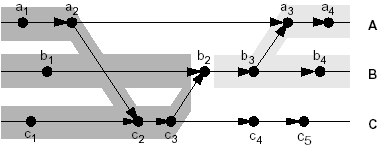
\includegraphics[width=0.45\textwidth]{img/img5.jpg}
	
	\caption{Структура зависимостей  событий}
	\label{fig:spire08}
\end{figure}

Следуя по стрелкам от события к событию с учётом взаимодействий, мы приходим к событиям, зависящим от начального. В отличии от последовательной программы, не все события в будущем могут быть достигнуты с помощью такого обхода, т.е. не все события причинно-зависимы. Рассмотрим событие b2. Все события в светло-серой области зависят от b2, но c4 и c5 не могут быть достигнуты из b2, так они не зависят от b2. Все события в тёмно-серой области влияют на b2, но все события, следующие за a2 и c3 могут быть отброшены при поиске причин b2.
При анализе трасс процессов с помощью таких зависимостей следует учесть, что:
1. необходимо знать положение каждого события локально внутри процесса;
2. должно быть возможно определить связанные пары событий в разных процессах
Эти требования могут быть удовлетворены, если исследуемая система предоставляет соответствующую информацию о событиях с сохранением её в трассе. При обработке таких трасс достаточным критерием для соответствия двух событий одному и тому же сообщению является одинаковое количество «пишущих» событий в одном процессе и «читающих» - в другом. В других случаях, например, при перекрывающихся  сообщениях, необходимо фиксировать дополнительную информацию, которая может быть использована для сопоставления пар событий. Примером такой информации могут служить номера пакетов в коммуникационных протоколах.
Анализ зависимостей в компьютерных системах означает следование по связанным событиям из конкретной точки, которая представляет собой интересное (нежелательное) поведение системы. Все инструкции программы, являющиеся причиной данного события являются кандидатами на оптимизацию. В параллельных системах с большим количеством процессов такое ограничение по предшествующим событиям позволяет сконцентрироваться на основных моментах, что приводит к значительному снижению затрат на анализ. 
\subsubsection{Сбор данных}
Учитывая сложность реальной вычислительной системы, не представляется возможным предсказать поведение системы во времени с помощью теоретических изысканий. По этой причине в большинстве инструментов программирования отсутствуют средства «планирования производительности». А те инструменты, в которые включён анализ производительности, дают лучшие результаты при профилировании. Профилирование оказывает большую помощь при программировании последовательных программ, при этом используется подход, основанный на измерениях. Т.е. определяется момент входа и выхода из каждой подпрограммы, подсчитывается количество вызовов каждой подпрограммы. Мониторинг делает шаг вперёд по отношению к простому измерению – маркеры событий вставляются в программный код в местах, предоставляющих определённый интерес, и достижение маркера может означать, что программа совершила определённые действия. С помощью этих средств программа может быть анализирована на разных уровнях абстракции, определяемых разметкой исходников.
\subsubsection{Время сбора данных}
Есть два разных подхода к определению моментов, когда информация о состоянии системы должна быть собрана профилировщиком. Традиционные методы используют временнОй подход, при котором информация непрерывно пишется по протоколу, схожему с медицинским оборудованием, или данные собираются с определённой частотой. Этот подход имеет право на жизнь при малой частоте сбора данных для получения общего вида поведения системы. Для получения информации о внутреннем поведении вычислительной системы необходима высокая частота сбора событий с одной стороны и длительный промежуток времени – с другой. При описанном подходе это приведёт к огромному потоку данных.
Событийный мониторинг позволяет уменьшить объём данных на несколько порядков. При этом на важных частях программы фиксируется больше событий, чем на остальных. Тем самым достигается необходимая пользователю картина о динамическом поведении системы. При этом подходе измерения выполняемой программы порождают компактный вид системы, отбрасывающий детали, ненужные для решения текущего вопроса.
\subsection{Технологии параллельного программирования}
Широкое распространение компьютеров  распределённой памятью определило и появление соответствующих систем программирования. Как правило, в таких системах отсутствует единое адресное пространство, и для обмена данными между параллельными процессами используется явная передача сообщений через коммуникационную среду. Отдельные процессы описываются с помощью традиционных языков программирования, а для организации их взаимодействия вводятся дополнительные функции. По этой причине практически все системы программирования, основанные на явной передачи сообщений, существуют не только в виде новых языков, а в виде интерфейсов и библиотек.
К настоящему времени примеров известных систем программирования на основе передачи сообщений накопилось довольно много: Shmem, Linda, PVM, MPI, PARMACS, P4, MPL, NX и др. В этом разделе рассмотрим наиболее популярные системы.
\subsubsection{Linda}
Идея построения системы Linda исключительно проста, а потому красива и очень привлекательна. Параллельная программа есть множество параллельных процессов, и каждый процесс работает согласно обычной последовательной программе. Все процессы имеют доступ к общей памяти, единицей хранения в которой является кортеж. Отсюда происходит и специальное название для общей памяти - пространство кортежей. Каждый кортеж это упорядоченная последовательность значений. 
\subsubsection{PVM (Parallel Virtual Machine)}
Параллельную виртуальную машину (PVM) можно определить как часть средств реального вычислительного комплекса (процессоры, память, периферийные устройства и т.д.), предназначенную для выполнения множества задач, участвующих в получении общего результата вычислений. В общем случае число задач может превосходить число процессоров, включенных в PVM.
\subsubsection{MPI (Message Passing Interface)}
Наиболее распространённой технологией программирования параллельных компьютеров м распределённой памятью в настоящее время является MPI. Стандарт MPI фиксирует интерфейс, который должны соблюдать как система программирования MPI на каждой вычислительной системе, так и пользователь при создании свих программ. Современные реализации чаще всего соответствуют стандарту MPI версии 1.1. В 1997-1998 годах появился стандарт MPI 2.0, значительно расширяющий функциональность предыдущей версии. Однако, до сих пор этот стандарт не получил широкого распространения.
MPI-программа – это множество параллельных взаимодействующих процессов. Все процессы порождаются один раз, образуя параллельную часть программы. В ходе выполнения MPI-программы порождение дополнительных процессов или уничтожение существующих не допускается.
Каждый процесс работает в своём адресном пространстве, никаких общих переменных или данных в MPI нет. Основным способом взаимодействия между процессами является явная посылка сообщений. Для локализации взаимодействий параллельных процессов программы можно создавать группы процессов, предоставляя им общую среду для общения – коммуникатор. Состав образуемых групп произволен. Группы могут полностью входить одна в другую, не пересекаться или пересекаться частично. При старте программы всегда считается, что все порождённые процессы работают в рамках всеобъемлющего коммуникатора. Этот коммуникатор существует всегда и служит для взаимодействия всех процессов MPI-программы.
Каждый процесс имеет уникальный атрибут номер процесса, который является целым неотрицательным числом. С помощью этого атрибута происходит значительная часть взаимодействия процессов между собой. 

%%% Local Variables:
%%% mode: latex
%%% TeX-master: "rpz"
%%% End:
